\documentclass[10pt,a4paper]{article}
\usepackage[utf8]{inputenc}
\usepackage[english]{babel}
\usepackage{amsmath}
\usepackage{amsfonts}
\usepackage{amssymb}
\usepackage{setspace}
\usepackage[pdftex]{graphicx}
\usepackage{url}
\usepackage{listings}
\usepackage{nameref}


\usepackage[round]{natbib}
\usepackage{bibentry}
\nobibliography*

\begin{document}
\pagenumbering{gobble} % switch off page numbering
\onehalfspacing 
\begin{titlepage}
\author{Michael Jungo\footnote{michael.jungo@unifr.ch} \\ 07-917-099 \\ Alexander Rüedlinger\footnote{alexander.rueedlinger@unifr.ch} \\ 08-129-710\\ }
\title{Report - Project 4 \\ \vspace{0.5em} }

\date{\today}
\maketitle
\end{titlepage}

\tableofcontents
\pagenumbering{roman} % switch on roman page numbering
\newpage
\pagenumbering{arabic} % switch oon arabic page numbers (and reset to 1)
\section{Introduction}
During the semester in the course blah 


\section{Challenge}
\section{Approach}


\section{Deployment}
A Raspberry Pi is a cheap credit-card sized single-board computer. There are two models available - model A and model B. For our purposes we used the model B which costs around 55 swiss francs. It includes a single 700 MHz ARM CPU, 512 megabytes of RAM, a Fast Ethernet (10/100 MB) LAN port and a SD card slot. The operating system and the user data are stored on a 8 GB SD flash card. 

\subsection{Cluster setup}
The cluster consists of six Raspberry Pi devices. Such a cluster is sometimes denoted as Beowulf cluster\footnote{A Beowulf cluster is a computer cluster of identical, commodity computers.} or as Bramble\footnote{See \url{http://elinux.org/Bramble}} in the Raspberry Pi community.

\begin{figure}[!htb]
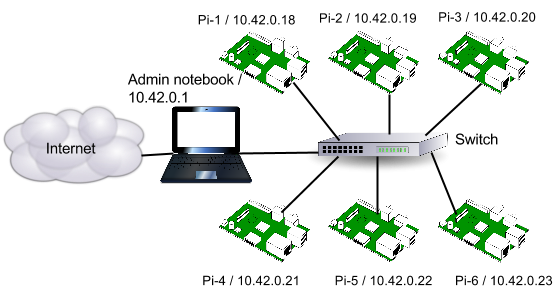
\includegraphics[scale=0.45]{png/pi_cluster.png} 
\centering
\caption{Raspberry Pi Cluster}
\end{figure}
For simplicity reasons we used a static network configuration. We connected each Raspberry Pi to a Gigabit Ethernet switch and assigned a static IP address to each host. 

The cluster is managed and controlled by a notebook. Additionally, we established a shared internet connection via the notbooks WiFi connection, allowing each host in the cluster to access the internet. 
By means of this network configuration we are able to run our Raspberry Pi cluster in the University network without the need to setup the internet connection for each host.


\section{Results}
\section{Conclusion}

As a final recommendation we would like to advocate for the use of Raspberry Pis in academia. They are great tool for learning how distributed systems work and they are very versatile, given you are not discouraged by the tinkering of the machines or the software that is required to get the most out of it's hardware.


\newpage
\addcontentsline{toc}{section}{References}
\bibliographystyle{plainnat}
\bibliography{biblio}
\nocite{*}


\end{document}
